\thispagestyle{empty}
\null
\vfill
\begin{center}
   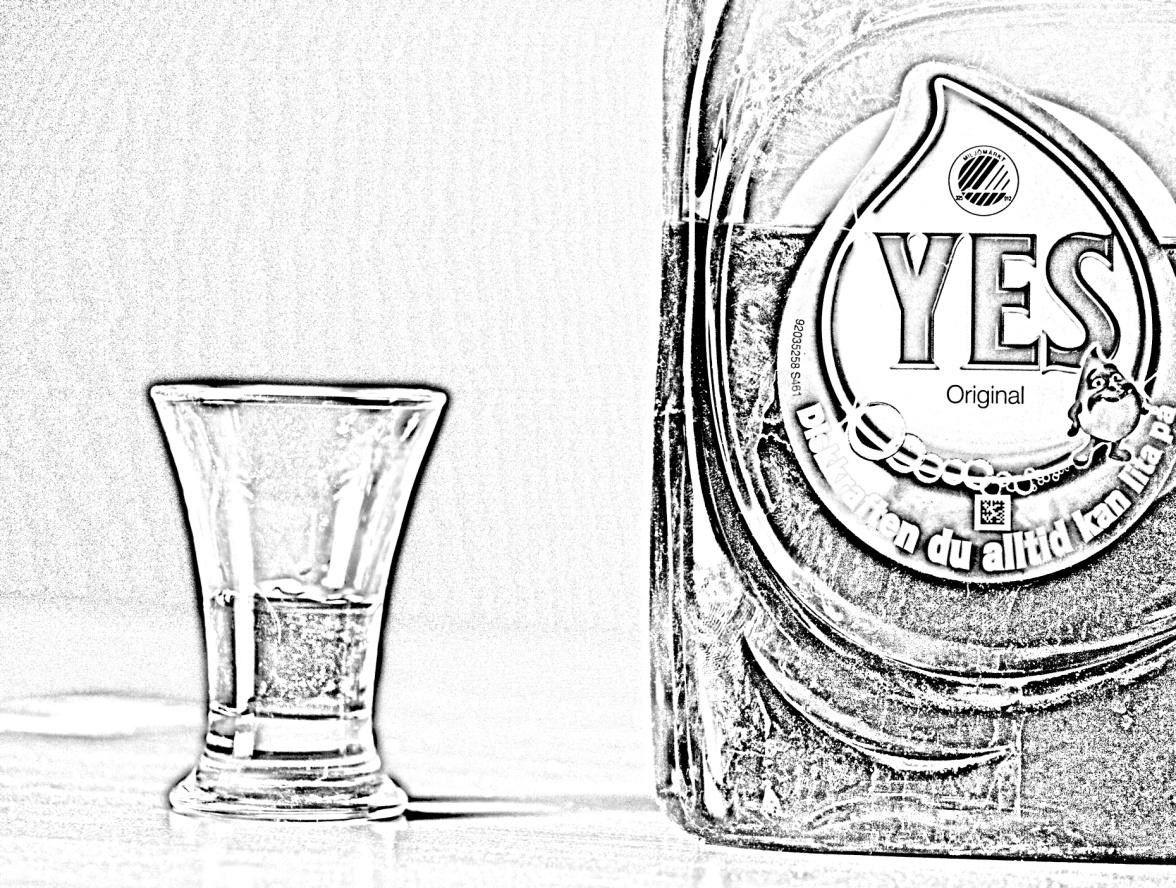
\includegraphics[width=1.0\textwidth]{res/drygavisor.jpg}
   \section{Dryga visor}
\end{center}
\vfill
\newpage

\begin{multicols}{2}
\subsection{Ebbe 1988}
\index[alfa]{Ebbe 1988}
\index[anfa]{Ebbe Ebbe Ebbe...}
\begin{parse lines}[\noindent]{#1\\}
Ebbe Ebbe Ebbe,
Ebbe, Ebbe.
Ebbe Ebbe Ebbe,
Ebbe, Ebbe.
Han ville bli polis.

Ebbe Ebbe Ebbe,
Ebbe,  Ebbe.
Ebbe Ebbe Ebbe,
Ebbe,  Ebbe.
Han samlade bevis.
\end{parse lines}

\subsection{Abbe 1989}
\index[alfa]{Abbe 1989}
\index[anfa]{Abbe Abbe Abbe...}
\begin{parse lines}[\noindent]{#1\\}
Abbe Abbe Abbe,
Abbe,  Abbe.
Abbe Abbe Abbe,
Abbe,  Abbe.
Var nollegeneral.

Abbe Abbe Abbe,
Abbe,  Abbe.
Abbe Abbe Abbe,
Abbe,  Abbe.
Han gjorde stor skandal.
\end{parse lines}

\subsection{Nubbe 1990}
\index[alfa]{Nubbe 1990}
\index[anfa]{Nubbe nubbe nubbe...}
\begin{parse lines}[\noindent]{#1\\}
Nubbe nubbe nubbe,
nubbe, nubbe.
Nubbe nubbe nubbe,
nubbe, nubbe.
Den är ljuv och sval.

Nubbe nubbe nubbe,
nubbe, nubbe.
Nubbe nubbe nubbe,
nubbe, nubbe.
Lyckan är total.
\end{parse lines}

\subsection{E:B 1991}
\index[alfa]{E:B 1991}
\index[anfa]{E:B E:B E:B...}
\begin{parse lines}[\noindent]{#1\\}
E:B E:B E:B,
E:B, E:B.
E:B E:B E:B,
E:B, E:B.
Reglerteknik på gång.

E:B E:B E:B,
E:B, E:B. E:B E:B E:B,
E:B, E:B.
Men salen var för trång
\end{parse lines}

\subsection{3-D 1992}
\index[alfa]{3-D 1992}
\index[anfa]{3-D 3-D 3-D...}
\begin{parse lines}[\noindent]{#1\\}
3-D 3-D 3-D
3-D, 3-D.
3-D 3-D 3-D
3-D, 3-D.
En extra dimension.

3-D 3-D 3-D
3-D, 3-D.
3-D 3-D 3-D
3-D, 3-D.
I vår television.
\end{parse lines}

\subsection{VG 1993}
\index[alfa]{VG 1993}
\index[anfa]{VG VG VG...}
\begin{parse lines}[\noindent]{#1\\}
VG VG VG
VG, VG.
VG VG VG
VG, VG.
Nu drar vi ut ett gäng.

VG VG VG
VG, VG.
VG VG VG
VG, VG.
En riktig nöjessväng.
\end{parse lines}

\subsection{BB 1994}
\index[alfa]{BB 1994}
\index[anfa]{BB BB BB...}
\begin{parse lines}[\noindent]{#1\\}
BB BB BB
BB, BB.
BB BB BB
BB, BB.
Sugklocka och tång.

BB BB BB
BB, BB.
BB BB BB
BB, BB.
Vi föddes på en gång!
\end{parse lines}

\subsection{VM 1995}
\index[alfa]{VM 1995}
\index[anfa]{VM SM AM...}
\begin{parse lines}[\noindent]{#1\\}
VM SM AM
EM, NM.
KM IM OM
FM, OS.
Medaljer tusenfalt!

VM SM AM
EM, NM.
KM IM OM
FM, OS.
Norge vinner allt!
\end{parse lines}

\begin{flushleft}
\subsection{Soap Addict 1996}
\index[alfa]{Soap Addict 1996}
\index[anfa]{Dallas, Falcon Crest och...}
\begin{parse lines}[\noindent]{#1\\}
Dallas, Falcon Crest och
Rederiet,
Bevvan, Skilda Världar,
det är givet.
Min fjärrkontroll går varm.
\end{parse lines}
\end{flushleft}
\begin{parse lines}[\noindent]{#1\\}
Varuhuset, Melrose
och Tre Kronor.
Grannar, Dynastin och,
Hem till gården.
Jag får tennisarm!
\end{parse lines}


\subsection{Björne 1997}
\index[alfa]{Björne 1997}
\index[anfa]{Björne Björne Björne...}
\begin{parse lines}[\noindent]{#1\\}
Björne Björne Björne
Björne, Björne.
Björne Björne Björne
Björne, Björne.
Vi ser hans magasin.

Björne Björne Björne
Björne, Björne.
Björne Björne Björne
Björne, Björne.
Fluffig, fet och fin!
\end{parse lines}

\subsection{Skvaller 1998}
\index[alfa]{Skvaller 1998}
\index[anfa]{Skvaller skvaller skvaller...}
\begin{parse lines}[\noindent]{#1\\}
Skvaller skvaller skvaller
skvaller, skvaller.
Skvaller skvaller skvaller
skvaller, skvaller.
Clinton var på glid.

Skvaller skvaller skvaller
skvaller, skvaller.
Skvaller skvaller skvaller
skvaller, skvaller.
Kungen är gravid!
\end{parse lines}


\subsection{B1 \& B2 1999}
\index[alfa]{B1 \& B2 1999}
\index[anfa]{B1 B1 B1...}
\begin{parse lines}[\noindent]{#1\\}
B1 B1 B1,
B1, B1.
B1 B1 B1,
B1, B1.
Vi står här och ler.

B2 B2 B2,
B2, B2.
B2 B2 B2,
B2, B2.
Vi ska skalas ner!
\end{parse lines}

\subsection{Kalle 2000}
\index[alfa]{Kalle 2000}
\index[anfa]{Kalle Kalle Kalle...}
\begin{parse lines}[\noindent]{#1\\}
Kalle Kalle Kalle,
Kalle, Kalle.
Kalle Kalle Kalle,
Kalle, Kalle.
Går på om en minut.

Kalle Kalle Kalle,
Kalle, Kalle.
Kalle Kalle Kalle,
Kalle, Kalle.
Det som vi sett förut!
\end{parse lines}

\vspace{-0.7cm}
\subsection{Ebbe 2001}
\index[alfa]{Ebbe 2001}
\index[anfa]{Killar killar killar...}
\begin{parse lines}[\noindent]{#1\\}
Killar killar killar
killar, killar.
Killar killar killar
killar, killar.
Killarna ska ut.

Tjejer tjejer tjejer,
tjejer, tjejer.
Tjejer tjejer tjejer,
tjejer, tjejer.
Tjejerna ska in.
\end{parse lines}
\vspace{-0.5cm}
\begin{flushleft}
\textit{2002 var Sångarstriden inställd. 2003 inkluderades ingen Ebbe-visa.}
\end{flushleft}
\subsection{Äggda 2004}
\index[alfa]{Äggda 2004}
\index[anfa]{Äggda Äggda Äggda...}
\begin{parse lines}[\noindent]{#1\\}
Äggda Äggda Äggda
Äggda, Äggda.
Äggda Äggda Äggda
Äggda, Äggda.
CF, SIF – Nej, Tack!

Äggda Äggda Äggda
Äggda, Äggda.
Äggda Äggda Äggda
Äggda, Äggda.
Äggen har sitt fack.
\end{parse lines}

\subsection{Sopor 2005}
\index[alfa]{Sopor 2005}
\index[anfa]{Sopor Sopor Sopor...}
\begin{parse lines}[\noindent]{#1\\}
Sopor Sopor Sopor,
Sopor, Sopor.
Sopor Sopor Sopor,
Sopor, Sopor.
Återvinns så lätt.

Sopor Sopor Sopor,
Sopor, Sopor.
Sopor Sopor Sopor,
Sopor, Sopor.
Skräpmat gör mig mätt!
\end{parse lines}

\subsection{Sjön Sjøn 2006}
\index[alfa]{Sjön Sjøn 2006}
\index[anfa]{Sjön Sjøn Sjön Sjøn Sjön Sjøn...}
\begin{parse lines}[\noindent]{#1\\}
Sjön Sjøn sjön Sjøn sjön Sjøn,
sjön Sjøn, sjön Sjøn.
Sjön Sjøn sjön Sjøn sjön Sjøn
sjön Sjøn, sjön Sjøn.
Vattnet som han drack.

Sjön Sjøn sjön Sjøn sjön Sjøn
sjön Sjøn, sjön Sjøn.
Sjön Sjøn sjön Sjøn sjön Sjøn
sjön Sjøn, sjön Sjøn.
Spydde ner en frack.
\end{parse lines}
\begin{flushleft}
\noindent \textit{Sångarstriden 2006 sköts fram till våren 2007. Sedermera sköts även Sångarstriden 2007 fram ett halvår. Data fick då dra sig ur på grund av krock med andra aktiviteter. Materialet sparades dock och användes 2008 istället.}
\end{flushleft}


\subsection{HB 2008}
\index[alfa]{HB 2008}
\index[anfa]{HB HB HB...}
\begin{parse lines}[\noindent]{#1\\}
HB HB HB,
HB, HB.
HB HB HB,
HB, HB.
När kärringen är svår.

HB HB HB,
HB, HB.
HB HB HB,
HB, HB.
Då tar jag mig en tår.
\end{parse lines}

\subsection{Clownens visa 2009}
\index[alfa]{Clownens visa 2009}
\index[anfa]{Ett å två å tre å...}
\begin{parse lines}[\noindent]{#1\\}
Ett å två å tre å,
fyra, fem, sex.
Sju å åtta, nio,
elva, tretton.
Ett mattegeni

1 + 2 är 4,
3 + 5 är ...
7 + 2 är 11,
18, 33!
Jag går ekonomi!
\end{parse lines}

\subsection{IP 2010}
\index[alfa]{IP 2010}
\index[anfa]{IP IP IP...}
\begin{parse lines}[\noindent]{#1\\}
IP IP IP,
IP, IP.
IP IP IP,
IP, IP.
Mitt favvoprotokoll

IP IP IP,
IP, IP.
IP IP IP,
IP, IP.
På adressen har jag koll
\end{parse lines}

\subsection{Tenta 2011}
\index[alfa]{Tenta 2011}
\index[anfa]{Tenta tenta tenta...}
\begin{parse lines}[\noindent]{#1\\}
Tenta tenta tenta,
tenta, tenta.
Tenta tenta tenta,
tenta, tenta.
Utan ett annex

Tenta tenta tenta,
tenta, tenta.
Tenta tenta tenta,
tenta, tenta.
Schemat blir komplex
\end{parse lines}


\subsection{Plugga 2012}
\index[alfa]{Plugga 2012}
\index[anfa]{Plugga plugga plugga...}
\begin{parse lines}[\noindent]{#1\\}
Plugga plugga plugga
plugga plugga
plugga plugga plugga
plugga plugga
36 veckor per år

Plugga plugga plugga
plugga plugga
plugga plugga plugga
plugga plugga
snart 40 om 'nåt år
\end{parse lines}
\vspace{-0.4cm}
\subsection{Ebbe 2013}
\index[alfa]{Ebbe 2013}
\index[anfa]{Jag har sett dig genom dina fönster...}
\begin{parse lines}[\noindent]{#1\\}
Jag har sett dig genom dina fönster
Jag kan se dina vanor, dina mönster
Vill du bli min fru?

Gå inte med honom
han är creepy
kom med mig istället
ner till Afrika
och rädda alla barn
\end{parse lines}
\vspace{-0.3cm}

\begin{flushleft}
\noindent\textit{Datatekniksektionen deltog inte i Sångarstriden 2014.}
\end{flushleft}

\subsection{Ebbe 2015}
\index[alfa]{Ebbe 2015}
\index[anfa]{Hen har sett dig genom...}
\begin{parse lines}[\noindent]{#1\\}
Hen har sett dig genom
tinder-appen
kom igen nu svara
öppna snappen
du gör vad som helst

Hen är ganska pryd och
riktigt kristen
ondheten hos dig du,
den e briiiisten
gå nu och bli frälst
\end{parse lines}
\vspace{-0.4cm}
\subsection{Sallad 2016}
\index[alfa]{Sallad 2016}
\index[anfa]{Sallad, sallad, sallad...}
\begin{parse lines}[\noindent]{#1\\}
Sallad, sallad, sallad
Sallad, sallad
Sallad, Salas, sallad
sallad, saaaallad
makten är för stor

Sallad, sallad, sallad
Sallad, sallad
Sallad, sallad, sallad
sallad, saaallad
sallad, sallad, sall.
\end{parse lines}

\subsection{Ketchup 2017}
\index[alfa]{Ketchup 2017}
\index[anfa]{Tar du denna tomat...}
\begin{parse lines}[\noindent]{#1\\}
Tar du denna tomat
Som din make
Ser till att älska honom
Hela livet ut
Det gör jag såklart

Tar du denna tomat
Som din maka
Ser till att älska henne
Hela livet ut
Verkligen absolut
\end{parse lines}
\vspace{-0.8cm}
\subsection{Ladok 2018}
\index[alfa]{Ladok 2018}
\index[anfa]{Välkomna till tentan här...}
\begin{parse lines}[\noindent]{#1\\}
Välkomna till tentan
här i kårgasque
Häng av jackan här o
stäng av telefonen.
Inga hjälpmedel.
Jag kan inte hitta
dig på listan.
Har du inte anmält
dig i laaaadok?
Ladok var ju stängt
Står du ej på listan,
får jag be dig
Lämna tentasalen,
ögonblickligen
Ge dig genast av!
\end{parse lines}
\end{multicols}








\subsection{Min gode vän Joel}
\textit{Mel: Trampa på gasen}\\
\index[alfa]{Min gode vän Joel}
\index[anfa]{Min gode vän Joel...}
\begin{parse lines}[\noindent]{#1\\}

Min gode vän Joel,
han är en glad kamrat,
Han har äpplen fram och en kulvert bak.

Min gode vän Joel,
han ser rätt lustig ut.
Man kan kalla honom Knut,
om man vill,
och det vill man.
\end{parse lines}


\subsection{Min gode vän Jor-El}
\textit{Mel: Trampa på gasen}\\
\index[alfa]{Min gode vän Jor-El}
\index[anfa]{Min gode vän Jor-El...}
\begin{parse lines}[\noindent]{#1\\}

Min gode vän Jor-El,
är far till Superman.
Super man som han blir man full som fan!
Min gode vän Jor-El,
han dricker supersprit,
men tål inte kryptonit!
Kastar upp
i raketen!
\end{parse lines}

\subsection{Bortom IT-samhället}
\textit{Mel: Trampa på gasen}\\
\index[alfa]{Bortom IT-samhället}
\index[anfa]{Usama bin Laden...}
\begin{parse lines}[\noindent]{#1\\}

Usama bin Laden
har ingen SMS,
ingen ICQ eller mailadress.
Usama bin Laden
tycks ha gått upp i rök,
man kan inte klicka 'Sök'
om man vill,
och det vill Bush (fortfarande)!
\end{parse lines}


\subsection{Den kuggade tentans visa}
\textit{Mel: Trampa på gasen}\\
\index[alfa]{Den kuggade tentans visa}
\index[anfa]{Jag kuggade tentan...}
\begin{parse lines}[\noindent]{#1\\}

Jag kuggade tentan
men det gör inte nått
för jag hade ändå inga pengar fått
för om man blir ratad
av hela CSN
får man ofta ringa hem
för att få lite pengar
\end{parse lines}

\vfill
\subsection{Jag pluggar på LU}
\textit{Mel: Trampa på gasen}\\
\index[alfa]{Jag pluggar på LU}
\index[anfa]{Jag pluggar på LU...}
\begin{parse lines}[\noindent]{#1\\}

Jag pluggar på LU,
och läser gratispoäng.
När ni gör er labb,
ligger jag i säng.

Jag pluggar på LU,
tar inga hårda tag.
Men ändå får jag bidrag,
från CSN, ja det får jag!
\end{parse lines}
\vfill
\subsection{Kalmarevisan}
\textit{Mel: Kalmare stad}\\
\index[alfa]{Kalmarevisan}
\index[anfa]{Uti Kalmare stad...}
\begin{parse lines}[\noindent]{#1\\}

Uti Kalmare stad,
ja där finns det ingen kvast
förrän lördagen.
Hej dick! Hej dack!
Jag slog i
och vi drack.
Hej dickom dickom dack,
hej dickom dickom dack.
För uti Kalmare stad,
ja där finns det ingen kvast
förrän lördagen.

$\vert\vert$: När som bonden kommer hem
kommer bondekvinnan ut :$\vert\vert$
Är så stor i sin trut.
Hej ...

$\vert\vert$: Var är pengarna du fått?
Jo, dem har jag supit opp :$\vert\vert$
uppå Kalmare slott.
Hej ...

$\vert\vert$: Jag ska klaga dig an
för vår Kronbefallningsman :$\vert\vert$
Och du ska få skam.
Hej ...

$\vert\vert$: Kronbefallningsmannen vår
satt på krogen igår :$\vert\vert$
och var full som ett får.
Hej ...
\end{parse lines}


\vfill
\subsection{Måsen}
\textit{Mel: När månen vandrar}\\
\index[alfa]{Måsen}
\index[anfa]{Det satt en mås på en klyvarbom...}
\begin{parse lines}[\noindent]{#1\\}

Det satt en mås på en klyvarbom,
och tom i krävan var kräket.
Och tungan lådde i skepparns gom
där han satt uti bleket.
Jag vill ha sill hördes måsen rope,
och skepparn svarte: Jag vill ha OP,
om blott jag får, om blott jag får.

Nu lyfter måsen från klyvarbom
och vinden spelar i tågen.
OP:n svalkat har skepparns gom.
Jag önskar blott att jag såg 'en.
Så nöjd och lycklig, den arme saten,
han sätter storsegel den krabaten.
Till sjöss han far, och halvan tar.

Den mås som satt på en klyvarbom,
den är nu död och begraven,
Och skepparn som drack en flaska rom,
han har nu drunknat i haven.
Så kan det gå om man fått för mycke,
om man för brännvin har fattat tycke.
Vi som har kvar, vi resten tar.
\end{parse lines}


\subsection{Anna: en disslåt}
\textit{Mel: När månen vandrar}\\
\index[alfa]{Anna: en disslåt}
\index[anfa]{Min kompis Anna, hon är en bot...}
\begin{parse lines}[\noindent]{#1\\}

Min kompis Anna, hon är en bot
Hon rensar upp i kanalen
Och varje gång jag hör hennes låt
Så får jag ont i analen.
Jag är så trött på den jävla låten
Kan någon vänlig själ banna boten?
Jag vete fan
Jag fick en ban
\end{parse lines}


\subsection{Att tenta matstat}
\textit{Mel: När månen vandrar}\\
\index[alfa]{Att tenta matstat}
\index[anfa]{Jag tänker tenta matstat nån gång...}
\begin{parse lines}[\noindent]{#1\\}

Jag tänker tenta matstat nån gång
jag tänker ta dom poängen
förra tentan blev inte lång
jag borde stannat i sängen
Den jävla kursen, den gör mig galen
Jag tror jag skyller, på karnevalen
och tar den sen i framtiden!
\end{parse lines}

\vfill
\subsection{Fotboll på Fäladen}
\textit{Mel: När månen vandrar}\\
\index[alfa]{Fotboll på Fäladen}
\index[anfa]{Det hände långt ut på Fäladen...}
\begin{parse lines}[\noindent]{#1\\}

Det hände långt ut på Fäladen,
jag skulle utöva fotboll.
Tog i för lite och tränaren,
han blev förtvivlad vid tolv-noll.

Jag våga inget, kapitulera,
men tränarn fortsatte propagera:
- Var ingen mes, det finns protes!
\end{parse lines}


\subsection{Groggen}
\textit{Mel: När månen vandrar}\\
\index[alfa]{Groggen}
\index[anfa]{Jag har nu blandat en helt ny grogg...}
\begin{parse lines}[\noindent]{#1\\}

Jag har nu blandat en helt ny grogg,
som gör mig full som en tunna.
Receptet skriver jag på min blogg,
så att andra ska kunna.
En Rom-o-cola, fast utan Cola
och mera rom, för vi ska ej snåla.
En god idé, den blir succé
\end{parse lines}

\vfill
\subsection{JAS:en}
\textit{Mel: När månen vandrar}\\
\index[alfa]{JAS:en}
\index[anfa]{Där flög en JAS över Västerbron...}
\begin{parse lines}[\noindent]{#1\\}

Där flög en JAS över Västerbron
Men styrsystemet var trasigt
Piloten sköt ut sig med kanon
För planet svängde så knasigt
``Jag vill ju uppåt, jag vill ju mer''
Men planet svarte: ``Jag vill ju ner
Mot alla hjon, på Västerbron''
\end{parse lines}


\subsection{Kompistipset}
\textit{Mel: När månen vandrar}\\
\index[alfa]{Kompistipset}
\index[anfa]{Min kompis Bosse, en bigamist...}
\begin{parse lines}[\noindent]{#1\\}

Min kompis Bosse, en bigamist,
tar alltid två öl i baren.
Han säger ``Allting kan verka trist,
ifall man blott bara tar en,
Nej, ta och skaffa dig en till fru å
be alltid bartendern om en duo.
Så skål min vän, och skål igen!''
\end{parse lines}

\vfill
\subsection{Mesen}
\textit{Mel: När månen vandrar}\\
\index[alfa]{Mesen}
\index[anfa]{Det satt en mes i en klyvarmast...}
\begin{parse lines}[\noindent]{#1\\}

Det satt en mes i en klyvarmast
där sågs han ragla och svaja
För trots att frön var hans enda last
var han full som en kaja
``Vad har du gjort!'' hördes skepparn stöna
och mesen svarte ``Jag rökte fröna
i egen holk, i egen holk.''
\end{parse lines}


\subsection{Moosen}
\textit{Mel: När månen vandrar}\\
\index[alfa]{Moosen}
\index[anfa]{Det satt en älg i en klyvartopp...}
\begin{parse lines}[\noindent]{#1\\}

Det satt en älg i en klyvartopp
Förklädd i älgjaktens månad
Han var befjädrad till horn och kropp
Och skepparn blev smått förvånad
``Jag är en mås, goa skepparn'' ljög den
förklädda älgen, därefter flög den
Mjukt föll han sen
På skepparen
\end{parse lines}

\vfill
\subsection{Musen}
\textit{Mel: När månen vandrar}\\
\index[alfa]{Musen}
\index[anfa]{Det satt en mus i en hushållsost...}
\begin{parse lines}[\noindent]{#1\\}

Det satt en mus i en hushållsost
och åt och åt utan måtta
tills osten blivit en mushåls-ost
och han en klotformad råtta
``Så bra'', sa musen, ``att va en fettboll,
nu kan jag rulla med hast åt rätt håll:
Ostindien! Ostindien!''
\end{parse lines}

\subsection{När månen vandrar}
\textit{Mel: När månen vandrar}\\
\index[alfa]{När månen vandrar}
\index[anfa]{När månen vandrar sin tysta ban...}
\begin{parse lines}[\noindent]{#1\\}

När månen vandrar sin tysta ban
Och tittar in genom rutan
Då tänker jag, att på ljusan dan,
då kan jag klara mig utan.
Då kan jag klara mig utan måne,
men utan Renat och utan Skåne?
Det vete fan, det vete fan.
\end{parse lines}

\newpage
\subsection{Röda havet}
\textit{Mel: Skrattvisa ur Orfeus i underjorden}\\
\index[alfa]{Röda havet}
\index[anfa]{Vi gingo ned till Röda Havet...}
\begin{parse lines}[\noindent]{#1\\}

Vi gingo ned till Röda Havet.
Vi lågo i där minst en kvart,
ja minst en kvart.
Men inte blev vi röda av 'et,
men Röda Havet det blev svart.

Men utav akvavit,
människan till kropp och själ
blir oskuldsfull och vit.
Men utav akvavit,
människan till kropp och själ
blir oskuldsfull och vit.
\end{parse lines}


\subsection{Finska viken}
\textit{Mel: Skrattvisa ur Orfeus i underjorden}\\
\index[alfa]{Finska viken}
\index[anfa]{Vi gingo ner till finska viken...}
\begin{parse lines}[\noindent]{#1\\}

Vi gingo ner till finska viken.
Vi lågo i där minst en kvart,
ja minst en kvart.
Men inte blev vi av med skiten,
men finska viken den blev svart.

Men utav akvavit…
\end{parse lines}


\subsection{Stadsparksdammen}
\textit{Mel: Skrattvisa ur Orfeus i underjorden}\\
\index[alfa]{Stadsparksdammen}
\index[anfa]{Vi gingo ner till stadsparksdammen...}
\begin{parse lines}[\noindent]{#1\\}

Vi gingo ner till stadsparksdammen.
Vi lågo i där minst en kvart,
ja minst en kvart.
Men inte blev vi av med skammen,
men stadsparksdammen den blev svart.

Men utav akvavit...
\end{parse lines}


\subsection{Systembolaget}
\textit{Mel: Skrattvisa ur Orfeus i underjorden}\\
\index[alfa]{Systembolaget}
\index[anfa]{Vi gingo ner till Systembolaget...}
\begin{parse lines}[\noindent]{#1\\}

Vi gingo ner till Systembolaget.
Vi stod i kö där minst en kvart,
ja minst en kvart.
Men inte blev vi fulla av det,
men systembolaget det gick back.

Men utav akvavit...
\end{parse lines}

\newpage
\subsection{Bastubadet}
\textit{Mel: Skrattvisa ur Orfeus i underjorden}\\
\index[alfa]{Bastubadet}
\index[anfa]{Vi gingo bort till bastubadet...}
\begin{parse lines}[\noindent]{#1\\}

Vi gingo bort till bastubadet
vi satt där inne minst en kvart
men satt för nära aggregatet
så stjärten den blev svart

Men utav akvavit...
\end{parse lines}


\subsection{Vi gingo ner till Edekvata}
\textit{Mel: Skrattvisa ur Orfeus i underjorden}\\
\index[alfa]{Vi gingo ner till Edekvata}
\index[anfa]{Vi gingo ned till Edekvata...}
\begin{parse lines}[\noindent]{#1\\}

Vi gingo ned till Edekvata.
Vi olja borden minst en kvart,
ja minst en kvart.
Men manualen den vi rata,
så Edekvata det blev svart.

Men utav akvavit...
\end{parse lines}

\newpage
\subsection{Lablokalen}
\textit{Mel: Skrattvisa ur Orfeus i underjorden}\\
\index[alfa]{Lablokalen}
\index[anfa]{Vi gingo ned till lablokalen...}
\begin{parse lines}[\noindent]{#1\\}

Vi gingo ned till lablokalen.
Vi var där inne minst en kvart,
ja minst en kvart.
Men inte blev vi av med kvalen,
men lablokalen den blev svart.

Men utav akvavit...
\end{parse lines}


\subsection{Lommabukten}
\textit{Mel: Skrattvisa ur Orfeus i underjorden}\\
\index[alfa]{Lommabukten}
\index[anfa]{Vi gingo ner till Lommabukten...}
\begin{parse lines}[\noindent]{#1\\}

Vi gingo ner till Lommabukten.
Vi lågo i där minst en kvart,
ja minst en kvart.
Men inte blev vi av med lukten,
men Lommabukten den blev svart.

Men utav akvavit...
\end{parse lines}

\vfill
\subsection{Karnevalen}
\textit{Mel: Skrattvisa ur Orfeus i underjorden}\\
\index[alfa]{Karnevalen}
\index[anfa]{Vi gingo ner till karnevalen...}
\begin{parse lines}[\noindent]{#1\\}

Vi gingo ner till karnevalen
och stod i kö där minst tre kvart.
Vi ville in i AF-salen
men inte fan kom vi nånvart.

För utav kösystem
blir det bara skit och allmänna problem.
För utav kösystem
blir det bara problem.

Och vi kom fram till kravallstaketet
och stod kvar där minst en kvart.
Men vi var fast i köhelvetet
så inte fan kom vi nånvart.

För utav kösystem…
\end{parse lines}

\newpage
